% Platform Economics: Full Standalone Lecture
% ~58 content frames across 8 sections
\documentclass[11pt,aspectratio=169]{beamer}
\usetheme{Madrid}

% ======================= PACKAGES =======================
\usepackage{graphicx}
\usepackage{booktabs}
\usepackage{adjustbox}
\usepackage{multicol}
\usepackage{amsmath}
\usepackage{amssymb}
\usepackage{tikz}
\usetikzlibrary{arrows,shapes,positioning,shadows,trees}
\usepackage{listings}
\usepackage{xcolor}

% ======================= COLOR DEFINITIONS =======================
% Primary color scheme: Blue/Teal for Digital Finance
\definecolor{dfblue}{RGB}{0,102,204}
\definecolor{dfteal}{RGB}{0,153,153}
\definecolor{dfcyan}{RGB}{51,187,204}
\definecolor{dflightblue}{RGB}{153,204,255}
\definecolor{dflightblue2}{RGB}{173,214,255}
\definecolor{dflightblue3}{RGB}{193,224,255}
\definecolor{dflightblue4}{RGB}{213,234,255}

% Accent colors for finance applications
\definecolor{dfgreen}{RGB}{44, 160, 44}
\definecolor{dfred}{RGB}{214, 39, 40}
\definecolor{dforange}{RGB}{255, 127, 14}
\definecolor{dfgray}{RGB}{127, 127, 127}

% Utility colors
\definecolor{lightgray}{RGB}{240, 240, 240}
\definecolor{midgray}{RGB}{180, 180, 180}
\definecolor{codebg}{RGB}{245, 245, 245}

% ======================= THEME CUSTOMIZATION =======================
% Apply Digital Finance color scheme to Madrid theme
\setbeamercolor{palette primary}{bg=dflightblue3,fg=dfblue}
\setbeamercolor{palette secondary}{bg=dflightblue2,fg=dfblue}
\setbeamercolor{palette tertiary}{bg=dfteal,fg=white}
\setbeamercolor{palette quaternary}{bg=dfblue,fg=white}

\setbeamercolor{structure}{fg=dfblue}
\setbeamercolor{section in toc}{fg=dfblue}
\setbeamercolor{subsection in toc}{fg=dfteal}
\setbeamercolor{title}{fg=dfblue}
\setbeamercolor{frametitle}{fg=dfblue,bg=dflightblue3}
\setbeamercolor{block title}{bg=dflightblue2,fg=dfblue}
\setbeamercolor{block body}{bg=dflightblue4,fg=black}

% Remove navigation symbols for cleaner look
\setbeamertemplate{navigation symbols}{}

% Clean itemize/enumerate
\setbeamertemplate{itemize items}[circle]
\setbeamertemplate{enumerate items}[default]

% Margins for readability
\setbeamersize{text margin left=8mm,text margin right=8mm}

% ======================= LISTINGS CONFIGURATION =======================
% Python code style
\lstdefinestyle{pythonstyle}{
    language=Python,
    basicstyle=\ttfamily\footnotesize,
    keywordstyle=\color{dfblue}\bfseries,
    stringstyle=\color{dforange},
    commentstyle=\color{dfgray}\itshape,
    numberstyle=\tiny\color{dfgray},
    numbers=left,
    numbersep=5pt,
    backgroundcolor=\color{codebg},
    showspaces=false,
    showstringspaces=false,
    showtabs=false,
    frame=single,
    rulecolor=\color{midgray},
    tabsize=4,
    captionpos=b,
    breaklines=true,
    breakatwhitespace=false,
    escapeinside={(*@}{@*)},
    xleftmargin=10pt,
    xrightmargin=10pt
}

% Solidity code style
\lstdefinestyle{soliditystyle}{
    language=Java, % closest approximation
    basicstyle=\ttfamily\footnotesize,
    keywordstyle=\color{dfteal}\bfseries,
    stringstyle=\color{dforange},
    commentstyle=\color{dfgray}\itshape,
    numberstyle=\tiny\color{dfgray},
    numbers=left,
    numbersep=5pt,
    backgroundcolor=\color{codebg},
    showspaces=false,
    showstringspaces=false,
    showtabs=false,
    frame=single,
    rulecolor=\color{midgray},
    tabsize=2,
    captionpos=b,
    breaklines=true,
    breakatwhitespace=false,
    escapeinside={(*@}{@*)},
    xleftmargin=10pt,
    xrightmargin=10pt,
    morekeywords={pragma, contract, function, returns, public, private, view, pure, payable, address, uint256, mapping, event, modifier}
}

% Inline code command
\newcommand{\code}[1]{\texttt{\color{dfblue}#1}}

% ======================= CUSTOM COMMANDS =======================
% Bottom annotation (Madrid-style)
\newcommand{\bottomnote}[1]{%
\vfill
\vspace{-2mm}
\textcolor{dflightblue2}{\rule{\textwidth}{0.4pt}}
\vspace{1mm}
\footnotesize
\textbf{#1}
}

% Compact list spacing
\newcommand{\compactlist}{%
\setlength{\itemsep}{0pt}%
\setlength{\parskip}{0pt}%
\setlength{\parsep}{0pt}%
}

% Chart placeholder
\newcommand{\chartplaceholder}[2][5cm]{%
\begin{center}
\begin{adjustbox}{max width=0.95\textwidth, max height=#1}
\framebox[\textwidth][c]{%
\rule{0pt}{#1}%
\textcolor{midgray}{[#2]}%
}
\end{adjustbox}
\end{center}
}

% ======================= FINANCE NOTATION MACROS =======================
% Probability and statistics
\newcommand{\E}{\mathbb{E}} % Expected value
\newcommand{\Var}{\mathrm{Var}} % Variance
\newcommand{\Cov}{\mathrm{Cov}} % Covariance
\newcommand{\Prob}{\mathbb{P}} % Probability

% Distributions
\newcommand{\Normal}{\mathcal{N}} % Normal distribution
\newcommand{\Uniform}{\mathcal{U}} % Uniform distribution

% Returns and prices
\newcommand{\Ret}{R} % Return
\newcommand{\LogRet}{r} % Log return
\newcommand{\Price}{S} % Price/Stock price
\newcommand{\Strike}{K} % Strike price

% Options and derivatives
\newcommand{\CallPrice}{C} % Call option price
\newcommand{\PutPrice}{P} % Put option price
\newcommand{\Greeks}[1]{\mathit{#1}} % Greek letters

% Risk measures
\newcommand{\VaR}{\mathrm{VaR}} % Value at Risk
\newcommand{\CVaR}{\mathrm{CVaR}} % Conditional VaR
\newcommand{\Sharpe}{\mathrm{SR}} % Sharpe Ratio

% Time series
\newcommand{\AR}{\mathrm{AR}} % Autoregressive
\newcommand{\MA}{\mathrm{MA}} % Moving average
\newcommand{\GARCH}{\mathrm{GARCH}} % GARCH

% Blockchain/Crypto
\newcommand{\Hash}{\mathrm{Hash}} % Hash function
\newcommand{\Block}{\mathcal{B}} % Block
\newcommand{\Chain}{\mathcal{C}} % Chain

% Real numbers, integers
\newcommand{\R}{\mathbb{R}}
\newcommand{\Z}{\mathbb{Z}}
\newcommand{\N}{\mathbb{N}}

% ======================= TIKZ STYLES =======================
% Styles for finance-related diagrams
\tikzstyle{process} = [rectangle, minimum width=3cm, minimum height=1cm, text centered, draw=dfblue, fill=dflightblue4, thick]
\tikzstyle{decision} = [diamond, minimum width=3cm, minimum height=1cm, text centered, draw=dfteal, fill=dflightblue4, thick]
\tikzstyle{arrow} = [thick,->,>=stealth,color=dfblue]
\tikzstyle{blockchain} = [rectangle, rounded corners, minimum width=2.5cm, minimum height=1cm, text centered, draw=dfteal, fill=dflightblue3, thick]
\tikzstyle{transaction} = [circle, minimum size=0.8cm, text centered, draw=dforange, fill=dflightblue4, thick]

% ======================= FOOTER TEMPLATE =======================
\setbeamertemplate{footline}{
    \hbox{\begin{beamercolorbox}[wd=\paperwidth,ht=2.5ex,dp=1ex,leftskip=.5em,rightskip=.5em]{author in head/foot}
    \tiny
    \textbf{Digital Finance} \hfill
    Joerg Osterrieder \hfill
    \insertdate \hfill
    Page \insertframenumber{} / \inserttotalframenumber
    \end{beamercolorbox}}
}

% ======================= SECTION DIVIDER TEMPLATE =======================
\AtBeginSection[]{
\begin{frame}[plain]
\vfill
\centering
\begin{beamercolorbox}[sep=12pt,center]{title}
\usebeamerfont{title}\LARGE\insertsection\par
\end{beamercolorbox}
\vfill
\end{frame}
}


% ======================= CUSTOM TIKZ STYLES =======================
\tikzstyle{platform} = [rectangle, rounded corners, minimum width=2.5cm,
    minimum height=1cm, draw=mlpurple, fill=mllavender3, thick, font=\small, text width=2.3cm, align=center]
\tikzstyle{side} = [rectangle, rounded corners, minimum width=2cm,
    minimum height=0.8cm, draw=dfteal, fill=dfteal!15, thick, font=\small, text width=1.8cm, align=center]
\tikzstyle{flywheel} = [circle, minimum size=1.8cm,
    draw=mlpurple, fill=mllavender4, thick, font=\scriptsize, text width=1.6cm, align=center]
\tikzstyle{deathnode} = [rectangle, rounded corners, minimum width=2cm,
    minimum height=0.7cm, draw=dfred, fill=dfred!15, thick, font=\scriptsize, text width=1.8cm, align=center]
\tikzstyle{sectionbox} = [rectangle, rounded corners, minimum width=1.8cm,
    minimum height=0.6cm, draw=mlpurple, fill=mllavender4, font=\tiny, text width=1.6cm, align=center]

% ======================= DOCUMENT INFO =======================
\title[Platform Economics]{Platform Economics: Theory, Strategy, and the Future of Digital Markets}
\subtitle{A Comprehensive Lecture}
\author{Joerg Osterrieder}
\institute{Digital Finance}
\date{}

\begin{document}

% =======================================================================
% FRAME 0: Title
% =======================================================================
\begin{frame}[plain]
\titlepage
\end{frame}

% =======================================================================
% FRAME 1: Learning Objectives
% =======================================================================
\begin{frame}{Learning Objectives}
\begin{block}{By the end of this lecture, you will be able to:}
\begin{enumerate}\compactlist
\item \textbf{Define} what a platform is and distinguish it from a traditional pipeline business
\item \textbf{Explain} network effects, two-sided markets, and critical mass using intuitive examples
\item \textbf{Analyze} platform launch strategies, pricing structures, and competitive dynamics
\item \textbf{Evaluate} platform business models using unit economics and sustainability frameworks
\item \textbf{Apply} platform economics concepts to real-world FinTech scenarios
\item \textbf{Synthesize} the implications of decentralization, regulation, and AI for the future of platforms
\end{enumerate}
\end{block}

\vspace{2mm}
\begin{alertblock}{Key Competency}
Analyze any platform business and assess whether it has a sustainable competitive advantage.
\end{alertblock}
\end{frame}

% =======================================================================
% FRAME 2: Lecture Roadmap
% =======================================================================
\begin{frame}{Lecture Roadmap}
\begin{center}
\begin{tikzpicture}[node distance=0.4cm and 0.6cm, >=stealth]
\node[sectionbox] (s1) {1. What is a\\Platform?};
\node[sectionbox, right=of s1] (s2) {2. Two-Sided\\Markets};
\node[sectionbox, right=of s2] (s3) {3. Strategy \&\\Competition};
\node[sectionbox, right=of s3] (s4) {4. Business\\Models};
\node[sectionbox, below=0.6cm of s1] (s5) {5. Data, Trust\\Governance};
\node[sectionbox, right=of s5] (s6) {6. Regulation\\Failures};
\node[sectionbox, right=of s6] (s7) {7. Platforms\\in Finance};
\node[sectionbox, right=of s7] (s8) {8. Synthesis\\Looking Ahead};
\draw[arrow] (s1) -- (s2);
\draw[arrow] (s2) -- (s3);
\draw[arrow] (s3) -- (s4);
\draw[arrow, dfteal] (s4.south) -- ++(0,-0.15) -| (s5.north);
\draw[arrow] (s5) -- (s6);
\draw[arrow] (s6) -- (s7);
\draw[arrow] (s7) -- (s8);
\end{tikzpicture}
\end{center}

\vspace{2mm}
\footnotesize
\begin{columns}[T]
\begin{column}{0.48\textwidth}
\begin{itemize}\compactlist
\item \textbf{Sections 1--4}: Foundations and theory
\item \textbf{Sections 5--6}: Governance, regulation, failures
\end{itemize}
\end{column}
\begin{column}{0.48\textwidth}
\begin{itemize}\compactlist
\item \textbf{Section 7}: FinTech applications
\item \textbf{Section 8}: Future directions and synthesis
\end{itemize}
\end{column}
\end{columns}

\bottomnote{This lecture expands on Topic 2.4 of the Digital Finance course. It is fully self-contained.}
\end{frame}

% #######################################################################
% SECTION 1: What is a Platform?
% #######################################################################
\section{What is a Platform?}

% =======================================================================
% FRAME 3: The Shift from Making to Connecting
% =======================================================================
\begin{frame}{The Shift from Making to Connecting}
\begin{alertblock}{A Provocative Question}
Why are some of the most valuable businesses ones that don't make anything?
\end{alertblock}

\vspace{2mm}
\begin{columns}[T]
\begin{column}{0.45\textwidth}
\textbf{\color{mlpurple}Pipeline Model}\\[2mm]
\footnotesize
Linear value chain: design $\rightarrow$ make $\rightarrow$ sell. The firm produces and the consumer buys.
\end{column}
\begin{column}{0.45\textwidth}
\textbf{\color{mlpurple}Platform Model}\\[2mm]
\footnotesize
Hub-and-spoke: the firm \emph{connects} participants who create value for each other.
\end{column}
\end{columns}

\vspace{3mm}
% TikZ DIAGRAM #1: Pipeline vs Platform
\begin{center}
\begin{tikzpicture}[node distance=0.8cm, >=stealth]
% Pipeline
\node[process, minimum width=1.5cm] (p1) {\scriptsize Design};
\node[process, minimum width=1.5cm, right=0.4cm of p1] (p2) {\scriptsize Make};
\node[process, minimum width=1.5cm, right=0.4cm of p2] (p3) {\scriptsize Sell};
\node[process, minimum width=1.5cm, right=0.4cm of p3] (p4) {\scriptsize Consumer};
\draw[arrow] (p1) -- (p2);
\draw[arrow] (p2) -- (p3);
\draw[arrow] (p3) -- (p4);
\node[above=0.1cm of p2] {\scriptsize \textbf{Pipeline}};

% Platform
\node[platform, below=1.2cm of p2.south east] (plat) {\scriptsize Platform};
\node[side, left=1cm of plat] (sa) {\scriptsize Side A};
\node[side, right=1cm of plat] (sb) {\scriptsize Side B};
\node[side, above=0.6cm of plat] (sc) {\scriptsize Side C};
\draw[arrow, dfteal] (sa) -- (plat);
\draw[arrow, dfteal] (plat) -- (sb);
\draw[arrow, dfteal] (sc) -- (plat);
\draw[arrow, dfteal] (plat) -- (sc);
\end{tikzpicture}
\end{center}

\vspace{-2mm}
\begin{exampleblock}{Insight}
\scriptsize The most powerful business model of our era is connecting people, not producing goods.
\end{exampleblock}
\end{frame}

% =======================================================================
% FRAME 4: Defining a Platform
% =======================================================================
\begin{frame}{Defining a Platform}
\begin{block}{Formal Definition}
\footnotesize
A \textbf{platform} is a business that creates value primarily by facilitating direct interactions between two or more distinct user groups (Parker, Van Alstyne, and Choudary, 2016).
\end{block}

\vspace{2mm}
\footnotesize
\textbf{\color{mlpurple}Four Key Characteristics:}
\begin{enumerate}\compactlist
\item \textbf{Two or more distinct sides} --- different types of participants
\item \textbf{Interdependence between sides} --- each side needs the other
\item \textbf{Platform orchestrates interaction} --- sets rules, provides infrastructure
\item \textbf{Value created by participants} --- the platform itself may produce nothing
\end{enumerate}

\vspace{2mm}
% TikZ DIAGRAM #2: Two-sided platform model
\begin{center}
\begin{tikzpicture}[node distance=1.5cm, >=stealth]
\node[side, minimum width=2.5cm] (a) {Side A\\{\tiny(e.g., Buyers)}};
\node[platform, right=1.5cm of a] (p) {Platform\\{\tiny Orchestrates}};
\node[side, right=1.5cm of p] (b) {Side B\\{\tiny(e.g., Sellers)}};
\draw[arrow, dfteal, thick] (a) -- node[above]{\tiny interaction} (p);
\draw[arrow, dfteal, thick] (p) -- node[above]{\tiny interaction} (b);
\draw[arrow, mlpurple, thick, dashed, bend left=30] (a) to node[below]{\tiny value exchange} (b);
\end{tikzpicture}
\end{center}

\bottomnote{\textbf{Two-sided market}: a market in which a platform serves two distinct user groups whose interactions generate value for both sides.}
\end{frame}

% =======================================================================
% FRAME 5: Pipeline vs Platform -- Detailed Comparison
% =======================================================================
\begin{frame}{Pipeline vs Platform --- Detailed Comparison}
\footnotesize
\begin{center}
\begin{tabular}{l p{4cm} p{4cm}}
\toprule
\textbf{Dimension} & \textbf{Pipeline} & \textbf{Platform} \\
\midrule
Value Creation & Firm produces goods/services & Participants create value for each other \\
Key Assets & Physical assets, inventory, IP & User base, data, network effects \\
Growth Pattern & Linear (more inputs $\rightarrow$ more output) & Non-linear (more users $\rightarrow$ more value per user) \\
Scalability & Limited by production capacity & Near-unlimited (digital matching) \\
Competition Basis & Product quality, cost efficiency & Network size, switching costs \\
Defensive Moat & Patents, brand, scale & Network effects, data advantage \\
Risk Profile & Inventory, operational risk & Platform trust, regulatory risk \\
Innovation Source & Internal R\&D & External developers and participants \\
\bottomrule
\end{tabular}
\end{center}

\vspace{2mm}
\begin{exampleblock}{Key Takeaway}
\footnotesize Platforms scale faster because adding users costs very little, yet each new user increases value for everyone else.
\end{exampleblock}
\end{frame}

% =======================================================================
% FRAME 6: Platform Taxonomy
% =======================================================================
\begin{frame}{Platform Taxonomy}
\footnotesize
% TikZ DIAGRAM #3: 2x2 matrix
\begin{center}
\begin{adjustbox}{max width=\textwidth}
\begin{tikzpicture}
% Axes
\draw[thick, ->] (0,0) -- (9,0) node[right]{\scriptsize \textbf{Innovation focus}};
\draw[thick, ->] (0,0) -- (0,5) node[above]{\scriptsize \textbf{Transaction focus}};

% Quadrants
\node[platform, minimum width=3.5cm, minimum height=1.5cm] at (2.5,3.5) {
\begin{tabular}{c}\textbf{Transaction}\\[-1mm]\tiny Facilitates exchanges\\[-1mm]\tiny (payment network)\end{tabular}};

\node[platform, minimum width=3.5cm, minimum height=1.5cm, fill=dfteal!15, draw=dfteal] at (6.5,3.5) {
\begin{tabular}{c}\textbf{Integrated}\\[-1mm]\tiny Transaction +\\[-1mm]\tiny innovation (ecosystem)\end{tabular}};

\node[platform, minimum width=3.5cm, minimum height=1.5cm, fill=mlorange!15, draw=mlorange] at (2.5,1.2) {
\begin{tabular}{c}\textbf{Investment}\\[-1mm]\tiny Capital providers\\[-1mm]\tiny meet seekers\end{tabular}};

\node[platform, minimum width=3.5cm, minimum height=1.5cm, fill=mlgreen!15, draw=mlgreen] at (6.5,1.2) {
\begin{tabular}{c}\textbf{Innovation}\\[-1mm]\tiny Foundation for\\[-1mm]\tiny third-party developers\end{tabular}};
\end{tikzpicture}
\end{adjustbox}
\end{center}

\vspace{1mm}
\begin{exampleblock}{Insight}
\scriptsize Many successful platforms evolve from one type toward ``Integrated,'' combining transactions with a developer ecosystem.
\end{exampleblock}
\end{frame}

% =======================================================================
% FRAME 7: Discussion -- Identifying Platforms
% =======================================================================
\begin{frame}{Discussion: Identifying Platforms}
\begin{alertblock}{Which of these are platforms? Which are pipelines?}
\footnotesize Classify each and explain your reasoning.
\end{alertblock}

\vspace{2mm}
\footnotesize
\begin{enumerate}\compactlist
\item An online marketplace for handmade goods
\item A traditional insurance company
\item A credit card network
\item A streaming video service
\item A peer-to-peer lending website
\item A conventional retail bank
\end{enumerate}

\vspace{3mm}
\begin{block}{Guiding Question}
\footnotesize What distinguishes a \emph{platform} from a \emph{pipeline that uses technology}? Is a bank that offers a mobile app a platform?
\end{block}

\vspace{2mm}
\begin{exampleblock}{Hint}
\scriptsize A platform requires \textbf{interdependent sides} and \textbf{value created by participants}. Technology alone does not make a platform.
\end{exampleblock}
\end{frame}

% #######################################################################
% SECTION 2: Two-Sided Markets and Network Effects
% #######################################################################
\section{Two-Sided Markets and Network Effects}

% =======================================================================
% FRAME 8: The Theory of Two-Sided Markets
% =======================================================================
\begin{frame}{The Theory of Two-Sided Markets}
\begin{block}{Academic Foundation}
\footnotesize
Rochet and Tirole (2003) formalized the economics of \textbf{two-sided markets}: a market is two-sided not simply because it has two customer groups, but because the platform can affect the volume of transactions by \emph{charging more to one side and reducing the charge to the other}.
\end{block}

\vspace{2mm}
\footnotesize
\textbf{\color{mlpurple}Key Insight:}
\begin{itemize}\compactlist
\item The \textbf{price structure} (how total price is divided between sides) matters, not just the \textbf{price level} (total price)
\item This is NOT just ``having two types of customers'' --- it is about cross-subsidization
\item The platform \textbf{internalizes network externalities}: it can make each side better off by managing the other side's participation
\end{itemize}

\vspace{2mm}
\begin{exampleblock}{Practical Example}
\scriptsize A card network charges merchants (money side) and rewards cardholders (subsidy side). If it charged both sides equally, fewer cardholders would join, reducing value for merchants.
\end{exampleblock}

\bottomnote{Rochet, J.-C. and Tirole, J. (2003). ``Platform Competition in Two-Sided Markets.'' \textit{Journal of the European Economic Association}, 1(4), 990--1029.}
\end{frame}

% =======================================================================
% FRAME 9: Network Effects -- The Core Engine
% =======================================================================
\begin{frame}{Network Effects --- The Core Engine}
\begin{alertblock}{Why does a payment network become more useful as more people join?}
\end{alertblock}

\vspace{2mm}
\footnotesize
\textbf{\color{mlpurple}Definition:} A \textbf{network effect} exists when the value of a product or service to one user depends on how many other users there are.

\vspace{3mm}
\begin{columns}[T]
\begin{column}{0.48\textwidth}
\textbf{Economies of Scale}\\(cost-side advantage)
\begin{itemize}\compactlist
\item More production $\rightarrow$ lower unit cost
\item Benefits the \emph{firm}, not directly the user
\item Linear and predictable
\item Example: manufacturing at volume
\end{itemize}
\end{column}
\begin{column}{0.48\textwidth}
\textbf{Network Effects}\\(demand-side advantage)
\begin{itemize}\compactlist
\item More users $\rightarrow$ more value per user
\item Benefits \emph{all participants}
\item Non-linear and self-reinforcing
\item Example: a peer payment app
\end{itemize}
\end{column}
\end{columns}

\vspace{3mm}
\begin{exampleblock}{Critical Distinction}
\scriptsize These are fundamentally different and often confused. Economies of scale reduce costs. Network effects increase demand. Both create barriers to entry, but through entirely different mechanisms.
\end{exampleblock}
\end{frame}

% =======================================================================
% FRAME 10: Types of Network Effects
% =======================================================================
\begin{frame}{Types of Network Effects}
\footnotesize
% TikZ DIAGRAM #4: Four types radiating from center
\begin{center}
\begin{tikzpicture}[node distance=1.2cm, >=stealth]
\node[platform, minimum width=2.5cm] (center) {\textbf{Network Effects}};

\node[process, minimum width=3cm, above left=0.8cm and 1cm of center, fill=mllavender3] (direct) {
\begin{tabular}{c}\textbf{Direct}\\[-1mm]\tiny Same-side\end{tabular}};
\node[process, minimum width=3cm, above right=0.8cm and 1cm of center, fill=dfteal!15, draw=dfteal] (indirect) {
\begin{tabular}{c}\textbf{Indirect}\\[-1mm]\tiny Cross-side\end{tabular}};
\node[process, minimum width=3cm, below left=0.8cm and 1cm of center, fill=mlgreen!15, draw=mlgreen] (data) {
\begin{tabular}{c}\textbf{Data}\\[-1mm]\tiny Usage-driven\end{tabular}};
\node[process, minimum width=3cm, below right=0.8cm and 1cm of center, fill=dfred!15, draw=dfred] (negative) {
\begin{tabular}{c}\textbf{Negative}\\[-1mm]\tiny Value-reducing\end{tabular}};

\draw[arrow, thick] (center) -- (direct);
\draw[arrow, thick] (center) -- (indirect);
\draw[arrow, thick] (center) -- (data);
\draw[arrow, thick, dfred] (center) -- (negative);
\end{tikzpicture}
\end{center}

\vspace{1mm}
\begin{columns}[T]
\begin{column}{0.48\textwidth}
\begin{itemize}\compactlist
\item \textbf{Direct}: More users on same side $\rightarrow$ more value\\{\scriptsize (messaging app: more friends = more useful)}
\item \textbf{Indirect}: More users on Side A $\rightarrow$ more value for Side B\\{\scriptsize (card network: more holders $\rightarrow$ more merchants)}
\end{itemize}
\end{column}
\begin{column}{0.48\textwidth}
\begin{itemize}\compactlist
\item \textbf{Data}: More usage $\rightarrow$ better algorithms $\rightarrow$ better product\\{\scriptsize (lending platform improves risk models)}
\item \textbf{Negative}: More users $\rightarrow$ \emph{less} value\\{\scriptsize (congestion, spam, fraud on a marketplace)}
\end{itemize}
\end{column}
\end{columns}
\end{frame}

% =======================================================================
% FRAME 11: Positive vs Negative Network Effects
% =======================================================================
\begin{frame}{Positive vs Negative Network Effects}
\footnotesize
\begin{columns}[T]
\begin{column}{0.48\textwidth}
\textbf{\color{mlgreen}Positive Network Effects}
\begin{itemize}\compactlist
\item Each new user \textbf{adds} value
\item Messaging app: more contacts = more useful
\item Payment network: wider acceptance = more convenient
\item Marketplace: more listings = better selection
\item Creates \textbf{virtuous cycle}: growth $\rightarrow$ value $\rightarrow$ more growth
\end{itemize}
\end{column}
\begin{column}{0.48\textwidth}
\textbf{\color{dfred}Negative Network Effects}
\begin{itemize}\compactlist
\item Each new user \textbf{reduces} value
\item Congestion: platform slows or degrades
\item Spam: unwanted content overwhelms quality
\item Fraud: bad actors erode trust
\item Creates \textbf{vicious cycle}: growth $\rightarrow$ degradation $\rightarrow$ departure
\end{itemize}
\end{column}
\end{columns}

\vspace{3mm}
\begin{alertblock}{Key Insight}
\footnotesize Platforms must actively manage negative network effects through curation, moderation, and trust mechanisms --- or growth itself becomes the enemy.
\end{alertblock}

\vspace{2mm}
\begin{exampleblock}{Example}
\scriptsize A marketplace that grows too fast without quality controls attracts fraudulent sellers, driving away buyers --- turning a positive network effect into a negative one.
\end{exampleblock}
\end{frame}

% =======================================================================
% FRAME 12: Network Value and Non-Linear Growth
% =======================================================================
\begin{frame}{Network Value and Non-Linear Growth}
\begin{alertblock}{Why do platforms seem to explode once they reach a certain size?}
\end{alertblock}

\vspace{2mm}
\footnotesize
In a network, value grows much faster than the number of users because each new user can interact with every existing user.

\vspace{1mm}
\textbf{Intuitive Example --- Group Chat:}
\begin{itemize}\compactlist
\item 3 friends = 3 possible conversations
\item Add 1 friend = 6 possible conversations
\item Add another = 10 possible conversations
\end{itemize}

\vspace{2mm}
% TikZ DIAGRAM #5: Linear vs Network value growth
\begin{center}
\begin{tikzpicture}
\begin{axis}[
    width=8cm, height=4cm,
    xlabel={\scriptsize Users}, ylabel={\scriptsize Value},
    xmin=0, xmax=10, ymin=0, ymax=50,
    xtick={0,2,4,6,8,10}, ytick={0,10,20,30,40,50},
    legend style={at={(0.02,0.98)}, anchor=north west, font=\tiny},
    grid=major, grid style={gray!20},
    tick label style={font=\tiny}
]
\addplot[mlpurple, thick, domain=0:10] {x*5};
\addlegendentry{Pipeline (linear)}
\addplot[dfteal, thick, domain=0:10] {x*(x-1)/2};
\addlegendentry{Network (non-linear)}
\end{axis}
\end{tikzpicture}
\end{center}

\scriptsize
\textit{Note: This is sometimes attributed to Metcalfe's Law, though the precise mathematical relationship is debated among researchers (Briscoe et al., 2006).}
\end{frame}

% =======================================================================
% FRAME 13: Critical Mass -- The Tipping Point
% =======================================================================
\begin{frame}{Critical Mass --- The Tipping Point}
\footnotesize
\textbf{\color{mlpurple}Definition:} \textbf{Critical mass} is the minimum number of users needed for a platform to become self-sustaining --- where organic growth exceeds churn without subsidies.

\vspace{2mm}
\begin{columns}[T]
\begin{column}{0.35\textwidth}
\textbf{Below Critical Mass:}
\begin{itemize}\compactlist
\item Users leave faster than they join
\item Weak value proposition
\item Requires heavy subsidies
\item High risk of failure
\end{itemize}

\textbf{Above Critical Mass:}
\begin{itemize}\compactlist
\item Organic growth dominates
\item Compounding effects
\item Winner-take-most begins
\item Sustainable economics
\end{itemize}
\end{column}
\begin{column}{0.60\textwidth}
% TikZ DIAGRAM #6: S-curve with critical mass line
\begin{center}
\begin{tikzpicture}
\begin{axis}[
    width=7cm, height=4.5cm,
    xlabel={\scriptsize Time}, ylabel={\scriptsize Users},
    xmin=0, xmax=10, ymin=0, ymax=100,
    xtick=\empty, ytick=\empty,
    grid=none,
    tick label style={font=\tiny}
]
\addplot[mlpurple, ultra thick, smooth, domain=0:10, samples=50] {100/(1+exp(-1.5*(x-4)))};
\draw[dashed, dfred, thick] (axis cs:4,0) -- (axis cs:4,100);
\node[font=\tiny, dfred] at (axis cs:4.2,85) {Critical Mass};
\node[font=\tiny, mlgray] at (axis cs:2,15) {Struggle Zone};
\node[font=\tiny, mlpurple] at (axis cs:7.5,85) {Dominance Zone};
\end{axis}
\end{tikzpicture}
\end{center}
\end{column}
\end{columns}

\vspace{1mm}
\begin{exampleblock}{Insight}
\scriptsize This is why platforms raise enormous amounts of capital --- to reach the tipping point before running out of money.
\end{exampleblock}
\end{frame}

% =======================================================================
% FRAME 14: When Markets "Tip" -- Winner-Take-Most
% =======================================================================
\begin{frame}{When Markets ``Tip'' --- Winner-Take-Most}
\footnotesize
\textbf{\color{mlpurple}Three conditions for a market to tip:}

\vspace{2mm}
\begin{enumerate}\compactlist
\item \textbf{Strong network effects} --- each new user significantly increases value for existing users
\item \textbf{High switching costs} --- leaving the dominant platform is costly (data, relationships, integration)
\item \textbf{Low multi-homing} --- using multiple competing platforms simultaneously is difficult or expensive
\end{enumerate}

\vspace{3mm}
\begin{columns}[T]
\begin{column}{0.48\textwidth}
\textbf{\color{mlpurple}Winner-Take-ALL} (rare)\\
\scriptsize Nearly 100\% market share. Happens when all three conditions are extreme.\\
Example: A dominant card network standard.
\end{column}
\begin{column}{0.48\textwidth}
\textbf{\color{dfteal}Winner-Take-MOST} (common)\\
\scriptsize Dominant player with 60--80\% share, smaller competitors persist.\\
Example: Most digital marketplaces.
\end{column}
\end{columns}

\vspace{3mm}
\begin{alertblock}{Diagnostic Question}
\footnotesize Does this market have the conditions to tip, or will competition persist?
\end{alertblock}

\bottomnote{Eisenmann, T., Parker, G., and Van Alstyne, M. (2006). ``Strategies for Two-Sided Markets.'' \textit{Harvard Business Review}, 84(10).}
\end{frame}

% =======================================================================
% FRAME 15: Multi-Homing -- The Competition Preserver
% =======================================================================
\begin{frame}{Multi-Homing --- The Competition Preserver}
\footnotesize
\textbf{\color{mlpurple}Definition:} \textbf{Multi-homing} means using multiple competing platforms simultaneously.

\vspace{3mm}
\begin{columns}[T]
\begin{column}{0.48\textwidth}
\textbf{When multi-homing is easy:}
\begin{itemize}\compactlist
\item Competition persists
\item No single winner
\item Pricing power limited
\item Platforms compete on price/quality
\item Examples: ride-sharing, food delivery, buy-now-pay-later
\end{itemize}
\end{column}
\begin{column}{0.48\textwidth}
\textbf{When multi-homing is hard:}
\begin{itemize}\compactlist
\item Market tips to dominance
\item Lock-in effects emerge
\item Pricing power increases
\item Platforms compete on network size
\item Examples: payment networks, enterprise software
\end{itemize}
\end{column}
\end{columns}

\vspace{3mm}
\begin{exampleblock}{Insight}
\footnotesize Platforms try to \textbf{increase} switching costs; regulators try to \textbf{decrease} them. This tension is central to platform strategy and policy.
\end{exampleblock}
\end{frame}

% =======================================================================
% FRAME 16: Self-Assessment: Network Effects
% =======================================================================
\begin{frame}{Self-Assessment: Network Effects}
\footnotesize
\textbf{Q1:} A peer-to-peer payment app grows in value as more of your friends join. This is an example of \rule{2cm}{0.4pt} network effects.\\
\begin{itemize}\compactlist
\item[(A)] Indirect \quad (B) \textbf{Direct $\checkmark$} \quad (C) Data \quad (D) Negative
\end{itemize}

\vspace{3mm}
\textbf{Q2:} Which of the following would PREVENT a market from tipping to winner-take-most?\\
\begin{itemize}\compactlist
\item[(A)] Strong network effects \quad (B) High switching costs
\item[(C)] \textbf{Low multi-homing costs $\checkmark$} \quad (D) Data advantages
\end{itemize}

\vspace{3mm}
\textbf{Q3:} A marketplace for freelance services grows rapidly but quality declines as unvetted providers flood in. This illustrates \rule{2cm}{0.4pt}.\\
\begin{itemize}\compactlist
\item[(A)] Direct effects \quad (B) Positive externalities
\item[(C)] \textbf{Negative network effects $\checkmark$} \quad (D) Critical mass
\end{itemize}
\end{frame}

% #######################################################################
% SECTION 3: Platform Strategy and Competition
% #######################################################################
\section{Platform Strategy and Competition}

% =======================================================================
% FRAME 17: The Chicken-and-Egg Problem
% =======================================================================
\begin{frame}{The Chicken-and-Egg Problem}
\begin{alertblock}{The Fundamental Launch Challenge}
\footnotesize How do you launch a platform when each side needs the other to exist first?
\end{alertblock}

\vspace{3mm}
% TikZ DIAGRAM #7: Chicken-and-egg death spiral
\begin{center}
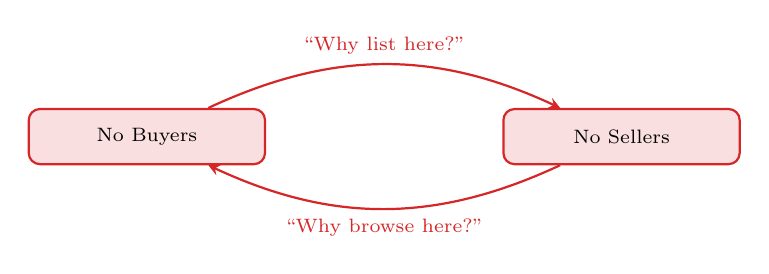
\begin{tikzpicture}[node distance=2cm, >=stealth]
\node[deathnode, minimum width=3cm] (nb) {No Buyers};
\node[deathnode, minimum width=3cm, right=3cm of nb] (ns) {No Sellers};
\draw[arrow, dfred, thick, bend left=25] (nb) to node[above, font=\scriptsize]{``Why list here?''} (ns);
\draw[arrow, dfred, thick, bend left=25] (ns) to node[below, font=\scriptsize]{``Why browse here?''} (nb);
\end{tikzpicture}
\end{center}

\vspace{2mm}
\footnotesize
\begin{itemize}\compactlist
\item Every two-sided platform faces this at launch
\item Without sellers, buyers see no value $\rightarrow$ they leave
\item Without buyers, sellers see no demand $\rightarrow$ they leave
\item The platform must \textbf{break the cycle} to survive
\end{itemize}

\begin{exampleblock}{Insight}
\scriptsize This is why the launch strategy is the single most critical decision for any new platform.
\end{exampleblock}
\end{frame}

% =======================================================================
% FRAME 18: Solving the Chicken-and-Egg -- Launch Strategies
% =======================================================================
\begin{frame}{Solving the Chicken-and-Egg: Six Launch Strategies}
\footnotesize
\begin{enumerate}\compactlist
\item \textbf{Subsidize one side}: Pay users to join (early payment apps gave sign-up bonuses)
\item \textbf{Single-player mode}: Make the product useful \emph{without} a network (an expense tracker that later becomes social)
\item \textbf{Seed supply}: Create initial content or supply yourself (a marketplace that curates its first listings)
\item \textbf{Piggyback on existing network}: Launch where users already gather (a payment widget embedded in an existing social platform)
\item \textbf{Marquee user strategy}: Attract one high-profile participant that draws the other side (a celebrity endorsement or anchor tenant)
\item \textbf{Micro-market strategy}: Dominate a small niche first, then expand (geographic, demographic, or vertical focus)
\end{enumerate}

\vspace{2mm}
\begin{exampleblock}{Insight}
\footnotesize The launch strategy chosen often shapes the platform's economics for years. A subsidy-heavy launch creates expectations of low prices. A niche-first launch creates a focused but loyal community.
\end{exampleblock}

\bottomnote{Evans, D. and Schmalensee, R. (2016). \textit{Matchmakers: The New Economics of Multisided Platforms}. Harvard Business Review Press.}
\end{frame}

% =======================================================================
% FRAME 19: Platform Pricing -- Subsidy Side vs Money Side
% =======================================================================
\begin{frame}{Platform Pricing: Subsidy Side vs Money Side}
\footnotesize
\begin{block}{Rochet-Tirole Pricing Insight}
\scriptsize In a two-sided market, the optimal price structure is NOT determined by cost allocation to each side, but by the relative demand elasticities. One side is more price-sensitive (subsidize them); the other side captures more value per user on the other side (charge them).
\end{block}

\vspace{2mm}
\begin{center}
\begin{tabular}{l l l}
\toprule
\textbf{Fee Type} & \textbf{Description} & \textbf{Example} \\
\midrule
\textbf{Access fee} & One-time or subscription to join & Annual card fee \\
\textbf{Usage fee} & Per-transaction charge & Merchant interchange fee \\
\textbf{Enhanced fee} & Premium features or placement & Promoted listings \\
\bottomrule
\end{tabular}
\end{center}

\vspace{2mm}
\textbf{\color{mlpurple}Common Patterns:}
\begin{itemize}\compactlist
\item Card networks: charge merchants (money side), subsidize cardholders (subsidy side)
\item Marketplaces: charge sellers a commission, offer free browsing to buyers
\item Social trading platforms: free for followers, charge expert traders a success fee
\end{itemize}

\begin{alertblock}{Key Principle}
\scriptsize ``Get the price-sensitive side in the door; charge the side that benefits most from their presence.''
\end{alertblock}
\end{frame}

% =======================================================================
% FRAME 20: Platform Competition -- Envelopment
% =======================================================================
\begin{frame}{Platform Competition: Envelopment}
\footnotesize
\textbf{\color{mlpurple}Definition:} \textbf{Platform envelopment} means entering a rival's market by bundling the rival's functionality into your own platform.

\vspace{3mm}
\textbf{How it works:}
\begin{enumerate}\compactlist
\item A platform in Market A has a large user base
\item It extends into Market B by adding Market B's features
\item Shared users and shared data lower the marginal cost of entry
\item The standalone Market B platform struggles to compete against a bundled offering
\end{enumerate}

\vspace{2mm}
\textbf{\color{mlpurple}Why it works:}
\begin{itemize}\compactlist
\item Shared users already trust the enveloping platform
\item Cross-platform data enables better personalization
\item Bundling increases switching costs for the combined offering
\end{itemize}

\vspace{2mm}
\begin{alertblock}{Competitive Implication}
\footnotesize The biggest competitive threat to a platform is often not a direct rival, but an adjacent platform that absorbs your functionality.
\end{alertblock}
\end{frame}

% =======================================================================
% FRAME 21: Platform Competition -- Additional Strategies
% =======================================================================
\begin{frame}{Platform Competition: Additional Strategies}
\footnotesize
\begin{center}
\begin{tabular}{p{2.5cm} p{4cm} p{3.5cm}}
\toprule
\textbf{Strategy} & \textbf{Description} & \textbf{Works Best When} \\
\midrule
\textbf{Bundling} & Combining multiple services to increase switching costs & Platform has adjacent capabilities \\
\textbf{Fork-and-improve} & Taking an open platform's design and building a better version & Rival is open-source or open-protocol \\
\textbf{Backward integration} & Platform starts producing its own supply & Supply quality is inconsistent \\
\textbf{Standards wars} & Competing to become the default interface or protocol & Market is early-stage, standards unset \\
\bottomrule
\end{tabular}
\end{center}

\vspace{2mm}
\begin{exampleblock}{FinTech Relevance}
\footnotesize Fork-and-improve is extremely common in DeFi: open-source smart contracts are routinely copied, modified, and redeployed as competing protocols with different incentive structures.
\end{exampleblock}
\end{frame}

% =======================================================================
% FRAME 22: Platform Governance and Trust
% =======================================================================
\begin{frame}{Platform Governance and Trust}
\footnotesize
Platforms must govern: \textbf{Who can participate?} \textbf{What behavior is allowed?} \textbf{How are disputes resolved?}

\vspace{2mm}
\textbf{\color{mlpurple}Three Governance Mechanisms:}
\begin{enumerate}\compactlist
\item \textbf{Ratings and reputation systems}: Buyer/seller reviews, trust scores, verified badges
\item \textbf{Algorithmic curation}: Quality scores, ranking algorithms, recommendation engines
\item \textbf{Rules and enforcement}: Terms of service, dispute resolution, fraud detection
\end{enumerate}

\vspace{2mm}
\begin{columns}[T]
\begin{column}{0.48\textwidth}
\textbf{\color{dfred}Too little governance:}
\begin{itemize}\compactlist
\item Fraud proliferates
\item Spam overwhelms quality
\item Trust collapses
\item Users flee
\end{itemize}
\end{column}
\begin{column}{0.48\textwidth}
\textbf{\color{dfred}Too much governance:}
\begin{itemize}\compactlist
\item Participation stifled
\item Innovation suppressed
\item Costs escalate
\item Users flee (different reason)
\end{itemize}
\end{column}
\end{columns}

\vspace{2mm}
\begin{exampleblock}{Insight}
\footnotesize ``Trust is the invisible product every platform sells.'' The governance dilemma is finding the balance.
\end{exampleblock}
\end{frame}

% =======================================================================
% FRAME 23: The Role of Data in Platform Competition
% =======================================================================
\begin{frame}{The Role of Data in Platform Competition}
\footnotesize
% TikZ DIAGRAM #8: Data flywheel cycle
\begin{center}
\begin{tikzpicture}[node distance=1.5cm, >=stealth]
\node[flywheel] (users) {More\\Users};
\node[flywheel, right=1.2cm of users] (data) {More\\Data};
\node[flywheel, below=1.2cm of data] (algo) {Better\\Algorithms};
\node[flywheel, left=1.2cm of algo] (exp) {Better\\Experience};
\draw[arrow, mlpurple, thick] (users) -- (data);
\draw[arrow, mlpurple, thick] (data) -- (algo);
\draw[arrow, mlpurple, thick] (algo) -- (exp);
\draw[arrow, mlpurple, thick] (exp) -- (users);
\node[font=\scriptsize\bfseries, mlpurple] at ($(users)!0.5!(algo)$) {Data Flywheel};
\end{tikzpicture}
\end{center}

\vspace{-1mm}
\scriptsize
\textbf{\color{mlpurple}Three competitive advantages:}
(1) \textbf{Personalization} --- better matching and pricing;
(2) \textbf{Fraud detection} --- more data = better anomaly detection;
(3) \textbf{Predictive capability} --- anticipating demand, risk, churn.

\textbf{Why this creates barriers:} New entrants start with zero data; the incumbent has years of compounding advantage.

\begin{exampleblock}{Key Takeaway}
\scriptsize The data flywheel is a \textbf{compounding moat} --- it gets stronger with time and nearly impossible to replicate.
\end{exampleblock}
\end{frame}

% =======================================================================
% FRAME 24: Discussion -- Platform Strategy
% =======================================================================
\begin{frame}{Discussion: Platform Strategy Scenario}
\footnotesize
\begin{block}{Scenario}
\scriptsize You are launching a new peer-to-peer lending platform in a market currently dominated by two established players. Both have strong data flywheels and moderate network effects.
\end{block}

\vspace{2mm}
\textbf{Discuss in pairs (3 minutes):}
\begin{enumerate}\compactlist
\item Which \textbf{launch strategy} would you choose and why?
\item Would you target the \textbf{subsidy side} (borrowers) or the \textbf{money side} (lenders) first?
\item How would you \textbf{differentiate} from the incumbents?
\item What is your \textbf{biggest risk}?
\end{enumerate}

\vspace{3mm}
\begin{alertblock}{Guiding Framework}
\scriptsize Think about: network effect strength, multi-homing costs, data advantage, regulatory barriers, and which side is more price-sensitive.
\end{alertblock}
\end{frame}

% #######################################################################
% SECTION 4: Platform Business Models
% #######################################################################
\section{Platform Business Models}

% =======================================================================
% FRAME 25: Platform Business Model Taxonomy
% =======================================================================
\begin{frame}{Platform Business Model Taxonomy}
\begin{alertblock}{How do platforms actually make money?}
\end{alertblock}

\vspace{2mm}
\footnotesize
\begin{center}
\begin{tabular}{l p{3.5cm} p{3cm} l}
\toprule
\textbf{Model} & \textbf{Revenue Source} & \textbf{Example Pattern} & \textbf{Scalability} \\
\midrule
\textbf{Commission} & \% of each transaction & Marketplace, payment processor & Very high \\
\textbf{Subscription} & Recurring access fee & B2B software platform & High \\
\textbf{Freemium} & Free basic, paid premium & Financial planning app & Medium \\
\textbf{Advertising} & Monetize attention/data & Comparison platform & High \\
\bottomrule
\end{tabular}
\end{center}

\vspace{2mm}
\begin{itemize}\compactlist
\item Most successful platforms \textbf{combine multiple models}
\item The choice depends on which side is the money side and which is the subsidy side
\item Revenue model must be \textbf{compatible with network effects} --- don't charge in ways that reduce participation
\end{itemize}
\end{frame}

% =======================================================================
% FRAME 26: Revenue Deep Dive -- Transaction Platforms
% =======================================================================
\begin{frame}{Revenue Deep Dive: Transaction Platforms}
\footnotesize
\textbf{\color{mlpurple}Transaction-based revenue in detail:}

\vspace{2mm}
\begin{itemize}\compactlist
\item \textbf{Take rate}: Percentage of gross merchandise value (typical range: 5--30\% depending on industry)
\item \textbf{Fixed fee per transaction}: Common in payments (small fixed amount + percentage)
\item \textbf{Interchange revenue}: Fees earned when cards are used for spending
\item \textbf{FX markups}: Premium on cross-border currency conversion
\end{itemize}

\vspace{2mm}
\begin{block}{The ``Rake'' Concept}
\footnotesize The \textbf{rake} (or \textbf{take rate}) is the percentage the platform keeps from each transaction. This is the single most important metric for a transaction platform.
\end{block}

\vspace{2mm}
\begin{exampleblock}{Scale Impact}
\scriptsize Even small changes in take rate have enormous impact at scale --- a one-percentage-point change on billions of transactions changes everything. This is why platforms guard their take rate fiercely.
\end{exampleblock}
\end{frame}

% =======================================================================
% FRAME 27: Revenue Deep Dive -- Subscription and Freemium
% =======================================================================
\begin{frame}{Revenue Deep Dive: Subscription and Freemium}
\footnotesize
\textbf{\color{mlpurple}Subscription Models:}
\begin{itemize}\compactlist
\item \textbf{Tiered pricing}: Free, basic, premium, enterprise levels
\item \textbf{Usage-based}: Pay per API call, per user, per transaction
\item \textbf{Bundled}: Platform access + multiple integrated services
\end{itemize}

\vspace{2mm}
\textbf{\color{mlpurple}Freemium Conversion Funnel:}
\begin{itemize}\compactlist
\item Large free user base $\rightarrow$ small percentage converts to paid
\item \textbf{Conversion rate}: Typically 2--5\% in consumer finance apps
\item \textbf{ARPU} (\textbf{Average Revenue Per User}): Total revenue / total users
\item \textbf{Churn rate}: Percentage of paying customers who cancel per period
\end{itemize}

\vspace{2mm}
\begin{alertblock}{Challenge}
\footnotesize Free users cost money to serve (infrastructure, support, fraud prevention). The conversion rate must justify the cost of serving non-paying users.
\end{alertblock}
\end{frame}

% =======================================================================
% FRAME 28: Revenue Deep Dive -- Data and Float
% =======================================================================
\begin{frame}{Revenue Deep Dive: Data and Float}
\footnotesize
\begin{columns}[T]
\begin{column}{0.48\textwidth}
\textbf{\color{mlpurple}Data Monetization:}
\begin{itemize}\compactlist
\item Selling aggregated, anonymized insights to third parties
\item \textbf{Payment for order flow} (\textbf{PFOF}): routing trades to market makers who pay for the flow
\item Cross-selling products using behavioral data
\item Privacy and ethical considerations are significant
\end{itemize}
\end{column}
\begin{column}{0.48\textwidth}
\textbf{\color{mlpurple}Float Income:}
\begin{itemize}\compactlist
\item Earning interest on funds held in transit
\item Deposit balances in customer accounts
\item Particularly valuable in high-interest-rate environments
\item Often an overlooked but substantial revenue source
\end{itemize}
\end{column}
\end{columns}

\vspace{3mm}
\begin{exampleblock}{Insight}
\footnotesize ``When you are not paying for the product, your data or your float likely \emph{is} the product.''
\end{exampleblock}

\bottomnote{\textbf{Float}: money held temporarily by a platform between receipt and disbursement, on which the platform earns interest.}
\end{frame}

% =======================================================================
% FRAME 29: Unit Economics -- The Health Check
% =======================================================================
\begin{frame}{Unit Economics --- The Health Check}
\footnotesize
\textbf{\color{mlpurple}Four Key Metrics (no math required):}

\vspace{2mm}
\begin{description}\compactlist
\item[\textbf{CAC}] \textbf{Customer Acquisition Cost}: Total marketing and sales spend to get one new customer
\item[\textbf{LTV}] \textbf{Lifetime Value}: Total expected revenue from one customer over their entire relationship
\item[\textbf{Payback Period}] Time until a customer ``pays back'' their acquisition cost through revenue
\item[\textbf{Churn Rate}] Percentage of customers who leave per period (monthly or annual)
\end{description}

\vspace{2mm}
\begin{block}{Health Indicators}
\footnotesize
\begin{itemize}\compactlist
\item LTV should be \textbf{several times} CAC (commonly a ratio of 3:1 or higher is considered healthy)
\item Payback period should be \textbf{within a reasonable timeframe} (under 18 months for consumer, under 24 for enterprise)
\item Churn should be \textbf{low and stable} (below 5\% monthly for consumer)
\end{itemize}
\end{block}

\begin{alertblock}{The Unit Economics Question}
\footnotesize Does each customer eventually pay back more than it cost to acquire them?
\end{alertblock}
\end{frame}

% =======================================================================
% FRAME 30: Venture Subsidies -- Real or Artificial Growth?
% =======================================================================
\begin{frame}{Venture Subsidies: Real or Artificial Growth?}
\footnotesize
\textbf{\color{mlpurple}The Blitzscaling Playbook:}
\begin{enumerate}\compactlist
\item Raise massive capital from venture investors
\item Subsidize below cost to attract users rapidly
\item Grow to critical mass before competitors
\item Turn off subsidies and monetize the network
\end{enumerate}

\vspace{2mm}
\begin{columns}[T]
\begin{column}{0.48\textwidth}
\textbf{\color{mlgreen}When it works:}
\begin{itemize}\compactlist
\item Market truly tips (strong network effects)
\item Network effects create lasting value
\item Switching costs prevent departure
\item Unit economics improve at scale
\end{itemize}
\end{column}
\begin{column}{0.48\textwidth}
\textbf{\color{dfred}When it fails:}
\begin{itemize}\compactlist
\item No real network effects
\item Multi-homing prevents lock-in
\item Competition never stops
\item Demand was artificial (price-driven)
\end{itemize}
\end{column}
\end{columns}

\vspace{2mm}
\begin{alertblock}{The ``Remove Subsidies'' Test}
\footnotesize Would customers stay at sustainable prices? If not, the growth is artificial.
\end{alertblock}
\end{frame}

% =======================================================================
% FRAME 31: Case Study -- Payment Processor Pricing Puzzle
% =======================================================================
\begin{frame}{Case Study: The Payment Processor Pricing Puzzle}
\footnotesize
\begin{block}{Scenario}
\scriptsize A major payment processing platform charges merchants a small percentage plus a flat fee per transaction. Consumers pay nothing. How do the economics work?
\end{block}

\vspace{2mm}
\begin{itemize}\compactlist
\item \textbf{Subsidy side}: Consumers pay nothing --- zero friction to adopt
\item \textbf{Network effect}: More consumers $\rightarrow$ merchants \emph{must} accept $\rightarrow$ more consumers
\item \textbf{Data flywheel}: Transaction data improves fraud detection $\rightarrow$ lower fraud $\rightarrow$ more merchants trust the platform
\item \textbf{Revenue composition}: Transaction fees (primary), premium merchant tools (secondary), data services (tertiary)
\end{itemize}

\vspace{2mm}
\begin{alertblock}{Discussion Question}
\footnotesize Why don't merchants rebel against the fees?
\end{alertblock}

\begin{exampleblock}{Answer}
\scriptsize The network effect is too strong --- refusing the dominant payment platform means losing customers. The \textbf{cost of not accepting} exceeds the \textbf{cost of the fee}.
\end{exampleblock}
\end{frame}

% =======================================================================
% FRAME 32: Self-Assessment: Business Models
% =======================================================================
\begin{frame}{Self-Assessment: Business Models}
\footnotesize
\textbf{Q1:} A FinTech app offers free basic accounts but charges for premium features like instant transfers and higher limits. This is a \rule{2cm}{0.4pt} model.\\[2mm]
\begin{itemize}\compactlist
\item[(A)] Commission \quad (B) Subscription \quad (C) \textbf{Freemium $\checkmark$} \quad (D) Advertising
\end{itemize}

\vspace{4mm}
\textbf{Q2:} A platform earns interest on customer funds held in transit between deposit and disbursement. This revenue source is called \rule{2cm}{0.4pt}.\\[2mm]
\begin{itemize}\compactlist
\item[(A)] Take rate \quad (B) \textbf{Float income $\checkmark$} \quad (C) Interchange \quad (D) PFOF
\end{itemize}

\vspace{4mm}
\textbf{Q3:} A lending platform has a Customer Acquisition Cost of \$50 and a Lifetime Value of \$30 per borrower. What does this indicate?\\[2mm]
\begin{itemize}\compactlist
\item[(A)] Healthy economics \quad (B) \textbf{Unsustainable unit economics $\checkmark$}
\item[(C)] Need more data \quad (D) Successful blitzscaling
\end{itemize}
\end{frame}

% #######################################################################
% SECTION 5: Data, Trust, and Platform Governance
% #######################################################################
\section{Data, Trust, and Platform Governance}

% =======================================================================
% FRAME 33: The Data Flywheel -- Compounding Advantage
% =======================================================================
\begin{frame}{The Data Flywheel --- Compounding Advantage}
\scriptsize
% TikZ DIAGRAM #9: Enhanced 5-node flywheel
\begin{center}
\begin{tikzpicture}[node distance=1.2cm, >=stealth]
\node[flywheel, minimum size=1.5cm] (trans) {More\\Transactions};
\node[flywheel, minimum size=1.5cm, right=1cm of trans] (data) {Richer\\Data};
\node[flywheel, minimum size=1.5cm, below right=0.8cm and 0.2cm of data] (models) {Better\\Models};
\node[flywheel, minimum size=1.5cm, below left=0.8cm and 0.2cm of trans] (exp) {Better\\Experience};
\node[flywheel, minimum size=1.5cm, below=0.6cm of $(models)!0.5!(exp)$] (trust) {More\\Trust};
\draw[arrow, mlpurple, thick] (trans) -- (data);
\draw[arrow, mlpurple, thick] (data) -- (models);
\draw[arrow, mlpurple, thick] (models) -- (trust);
\draw[arrow, mlpurple, thick] (trust) -- (exp);
\draw[arrow, mlpurple, thick] (exp) -- (trans);
\end{tikzpicture}
\end{center}

\vspace{-1mm}
\textbf{\color{mlpurple}Two flywheel examples:}
\begin{itemize}\compactlist
\item \textbf{Payments}: More transactions $\rightarrow$ more data $\rightarrow$ better fraud detection $\rightarrow$ fewer false declines $\rightarrow$ more merchants
\item \textbf{Lending}: More applications $\rightarrow$ better risk models $\rightarrow$ more accurate pricing $\rightarrow$ better borrowers $\rightarrow$ more data
\end{itemize}

\vspace{-1mm}
\begin{exampleblock}{Why new entrants struggle}
\scriptsize The data advantage \textbf{compounds over years}. Replicating a decade of accumulated data is nearly impossible.
\end{exampleblock}
\end{frame}

% =======================================================================
% FRAME 34: AI-Driven Network Effects
% =======================================================================
\begin{frame}{AI-Driven Network Effects}
\footnotesize
\textbf{\color{mlpurple}A new category beyond traditional network effects:}

\vspace{2mm}
\begin{itemize}\compactlist
\item AI/ML models improve with more training data (supervised learning on transaction patterns)
\item Better AI $\rightarrow$ better product $\rightarrow$ more users $\rightarrow$ more data $\rightarrow$ better AI
\item This creates a \textbf{``data moat''} that is extremely difficult to breach
\end{itemize}

\vspace{3mm}
\textbf{\color{mlpurple}Three AI applications in platform economics:}

\vspace{2mm}
\begin{enumerate}\compactlist
\item \textbf{Matching}: Better buyer-seller matching on marketplaces; better borrower-lender matching on lending platforms
\item \textbf{Pricing}: Dynamic pricing based on demand patterns; personalized interest rates and insurance premiums
\item \textbf{Risk assessment}: Real-time fraud detection across millions of transactions; automated credit scoring using alternative data
\end{enumerate}

\vspace{2mm}
\begin{alertblock}{Implication}
\footnotesize AI amplifies data network effects. As AI becomes more central to platform operations, the data advantage of incumbents becomes even more formidable.
\end{alertblock}
\end{frame}

% =======================================================================
% FRAME 35: Trust as Platform Infrastructure
% =======================================================================
\begin{frame}{Trust as Platform Infrastructure}
\footnotesize
\textbf{\color{mlpurple}Three Layers of Trust:}

\vspace{2mm}
\begin{enumerate}\compactlist
\item \textbf{Institutional trust}: Regulation, licensing, deposit insurance, legal recourse\\
{\scriptsize The traditional approach --- expensive and slow but well-understood}
\item \textbf{Peer trust}: Ratings, reviews, reputation scores, verified identities\\
{\scriptsize The platform approach --- fast and scalable but gameable}
\item \textbf{Algorithmic trust}: Smart contracts, automated escrow, on-chain verification\\
{\scriptsize The crypto approach --- trustless execution but limited flexibility}
\end{enumerate}

\vspace{3mm}
\begin{columns}[T]
\begin{column}{0.55\textwidth}
\textbf{Trust failures cascade:} One bad actor on a marketplace can damage trust for \emph{all} sellers. A single security breach can destroy years of reputation.
\end{column}
\begin{column}{0.40\textwidth}
\begin{exampleblock}{Insight}
\scriptsize ``Building trust is expensive and slow. Destroying it is instant.''
\end{exampleblock}
\end{column}
\end{columns}
\end{frame}

% =======================================================================
% FRAME 36: Platform Governance Challenges
% =======================================================================
\begin{frame}{Platform Governance Challenges}
\footnotesize
\textbf{\color{mlpurple}The Moderation Dilemma:} Who decides what is acceptable? How much control is appropriate?

\vspace{2mm}
\begin{center}
\begin{tabular}{p{2.5cm} p{3.5cm} p{3.5cm}}
\toprule
\textbf{Model} & \textbf{How It Works} & \textbf{Trade-off} \\
\midrule
\textbf{Centralized} & Platform sets rules unilaterally & Fast but potentially arbitrary \\
\textbf{Community} & Users vote on rules and policies (DAOs) & Democratic but slow, vulnerable to capture \\
\textbf{Algorithmic} & Rules encoded in code (smart contracts) & Consistent but inflexible \\
\bottomrule
\end{tabular}
\end{center}

\vspace{2mm}
\begin{alertblock}{The Paradox}
\footnotesize Users want \textbf{freedom} but also \textbf{safety}. Too much of either fails. The governance challenge is finding the balance that maximizes participation while minimizing harm.
\end{alertblock}

\vspace{1mm}
\begin{exampleblock}{Connection to Regulation}
\scriptsize When platforms fail to self-govern effectively, regulators step in with mandatory rules --- often blunter and more restrictive than what the platform could have implemented itself.
\end{exampleblock}
\end{frame}

% =======================================================================
% FRAME 37: Platform Power and Concentration
% =======================================================================
\begin{frame}{Platform Power and Concentration}
\footnotesize
\textbf{\color{mlpurple}Sources of Platform Power:}
\begin{itemize}\compactlist
\item User data and behavioral insights
\item Switching costs and lock-in effects
\item Network effects creating natural monopolies
\item Algorithmic control over visibility and access
\end{itemize}

\vspace{2mm}
\textbf{\color{mlpurple}Manifestations of Platform Power:}
\begin{description}\compactlist
\item[\textbf{Gatekeeper power}] Controlling access to a market (app stores, payment networks, lending marketplaces)
\item[\textbf{Information asymmetry}] Platform knows more about both sides than either side knows about itself
\item[\textbf{Self-preferencing}] Platform promotes its own products over third-party alternatives
\item[\textbf{Algorithmic manipulation}] Changing ranking algorithms to favor platform interests
\end{description}

\vspace{2mm}
\begin{alertblock}{Why This Matters}
\footnotesize This concentration of power is the core concern driving platform regulation worldwide. When a platform becomes the only gateway to a market, it becomes a de facto regulator itself.
\end{alertblock}
\end{frame}

% =======================================================================
% FRAME 38: Discussion -- Trust and Governance
% =======================================================================
\begin{frame}{Discussion: Trust and Governance Scenario}
\footnotesize
\begin{block}{Scenario}
\scriptsize A financial marketplace platform discovers that 5\% of its lenders are providing misleading information about their loan terms. Removing them would reduce marketplace supply significantly.
\end{block}

\vspace{2mm}
\textbf{Discuss (3 minutes):}
\begin{enumerate}\compactlist
\item What should the platform do? Remove all misleading lenders immediately, or phase them out gradually?
\item Who bears the cost of this governance failure --- the platform, the borrowers, or the honest lenders?
\item Should the platform have caught this earlier? How?
\item Would a decentralized (DAO-based) governance model handle this better or worse?
\end{enumerate}

\vspace{2mm}
\begin{alertblock}{Key Tension}
\footnotesize Short-term supply loss vs long-term trust. Most platforms that choose short-term supply over long-term trust eventually face a larger crisis.
\end{alertblock}
\end{frame}

% #######################################################################
% SECTION 6: Regulation and Platform Failures
% #######################################################################
\section{Regulation and Platform Failures}

% =======================================================================
% FRAME 39: Why Regulate Platforms?
% =======================================================================
\begin{frame}{Why Regulate Platforms?}
\footnotesize
\textbf{\color{mlpurple}Four Market Failure Arguments:}

\vspace{2mm}
\begin{enumerate}\compactlist
\item \textbf{Market power}: Winner-take-most dynamics create near-monopolies that can exploit users
\item \textbf{Information asymmetry}: Platforms have superior information about users, transactions, and market conditions
\item \textbf{Externalities}: Platform decisions affect millions of users, businesses, and the broader economy
\item \textbf{Systemic risk}: Financial platforms can create cascading failures that threaten financial stability
\end{enumerate}

\vspace{3mm}
\begin{alertblock}{The Regulator's Dilemma}
\footnotesize Regulate too early $\rightarrow$ stifle innovation and prevent beneficial platforms from emerging. Regulate too late $\rightarrow$ entrenched power that is very difficult to dislodge.
\end{alertblock}

\vspace{2mm}
\begin{exampleblock}{Financial Context}
\scriptsize Financial platforms face additional regulatory scrutiny because they handle people's money, credit, and financial data --- the stakes of failure are higher than in most other platform markets.
\end{exampleblock}
\end{frame}

% =======================================================================
% FRAME 40: Regulatory Approaches to Platforms
% =======================================================================
\begin{frame}{Regulatory Approaches to Platforms}
\footnotesize
\begin{center}
\begin{tabular}{p{2.5cm} p{3.5cm} p{3.5cm}}
\toprule
\textbf{Approach} & \textbf{How It Works} & \textbf{Example Concept} \\
\midrule
\textbf{Competition law} (ex-post) & Traditional antitrust: intervene after harm & Merger review, abuse of dominance \\
\textbf{Gatekeeper rules} (ex-ante) & New rules for designated large platforms & EU DMA/DSA framework concept \\
\textbf{Interoperability mandates} & Force data portability and switching & PSD2/Open Banking approach \\
\bottomrule
\end{tabular}
\end{center}

\vspace{2mm}
\textbf{\color{mlpurple}Key Regulatory Concepts:}
\begin{itemize}\compactlist
\item \textbf{Gatekeeper designation}: Based on size, user counts, and market position
\item \textbf{Obligations}: Data portability, interoperability, prohibition of self-preferencing
\item \textbf{Trend}: Regulation is shifting from \emph{reactive} (fix after harm) to \emph{proactive} (prevent by design)
\end{itemize}

\begin{exampleblock}{Insight}
\scriptsize Open Banking regulations (requiring banks to share data via APIs) are a direct example of interoperability mandates designed to reduce platform lock-in in financial services.
\end{exampleblock}
\end{frame}

% =======================================================================
% FRAME 41: Regulation as Competitive Moat
% =======================================================================
\begin{frame}{Regulation as Competitive Moat}
\footnotesize
\begin{alertblock}{The Paradox}
\footnotesize Regulation intended to protect consumers can paradoxically help established platforms by raising barriers to entry.
\end{alertblock}

\vspace{2mm}
\textbf{\color{mlpurple}How compliance becomes a barrier:}
\begin{itemize}\compactlist
\item Banking charters, money transmitter licenses, insurance licenses are expensive to obtain
\item Compliance infrastructure (KYC, AML, reporting) costs millions to build
\item Established players have already invested; new entrants must start from scratch
\end{itemize}

\vspace{2mm}
\textbf{\color{mlpurple}Three Strategies for New Entrants:}
\begin{enumerate}\compactlist
\item \textbf{Rent}: Use a Banking-as-a-Service partner's license (fast but dependent)
\item \textbf{Obtain}: Apply for your own license (slow but independent)
\item \textbf{Avoid}: Operate in an unregulated niche or jurisdiction (risky but cheap)
\end{enumerate}

\vspace{2mm}
\begin{exampleblock}{Insight}
\footnotesize ``Once compliant, regulation becomes a competitive barrier. Expensive to achieve, powerful to hold.'' The double edge: what protects today can restrict tomorrow.
\end{exampleblock}
\end{frame}

% =======================================================================
% FRAME 42: Platform Failures -- The Death Spiral
% =======================================================================
\begin{frame}{Platform Failures: The Death Spiral}
\scriptsize
\begin{columns}[T]
\begin{column}{0.38\textwidth}
% TikZ DIAGRAM #10: Death spiral
\begin{center}
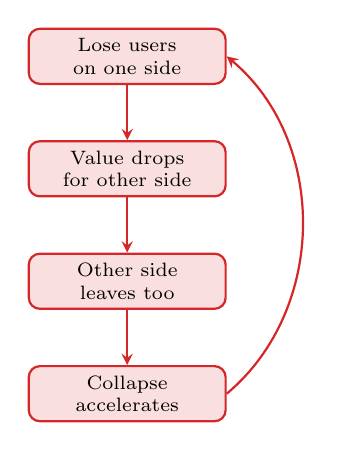
\begin{tikzpicture}[node distance=0.7cm, >=stealth]
\node[deathnode, minimum width=2.5cm] (lose) {Lose users\\on one side};
\node[deathnode, minimum width=2.5cm, below=of lose] (value) {Value drops\\for other side};
\node[deathnode, minimum width=2.5cm, below=of value] (leave) {Other side\\leaves too};
\node[deathnode, minimum width=2.5cm, below=of leave] (accel) {Collapse\\accelerates};
\draw[arrow, dfred, thick] (lose) -- (value);
\draw[arrow, dfred, thick] (value) -- (leave);
\draw[arrow, dfred, thick] (leave) -- (accel);
\draw[arrow, dfred, thick, bend right=50] (accel.east) to (lose.east);
\end{tikzpicture}
\end{center}
\end{column}
\begin{column}{0.58\textwidth}
\begin{alertblock}{What makes a platform collapse?}
\scriptsize The death spiral: losing users on one side reduces value for the other side, causing them to leave too.
\end{alertblock}

\vspace{1mm}
\textbf{\color{mlpurple}Six failure causes:}
\begin{enumerate}\compactlist
\item \textbf{Trust collapse}: Fraud, security breach, privacy scandal
\item \textbf{Negative network effects}: Growth outpaces quality controls
\item \textbf{Disintermediation}: Users bypass the platform to avoid fees
\item \textbf{Competitor envelopment}: Larger platform absorbs your functionality
\item \textbf{Regulatory shutdown}: Model restricted or banned
\item \textbf{Technology obsolescence}: Underlying tech surpassed
\end{enumerate}
\end{column}
\end{columns}
\end{frame}

% =======================================================================
% FRAME 43: Case Study -- Marketplace Lending Collapse
% =======================================================================
\begin{frame}{Case Study: The Marketplace Lending Collapse}
\footnotesize
\begin{block}{Generic Case}
\scriptsize Several marketplace lending platforms experienced severe distress during economic downturns.
\end{block}

\vspace{2mm}
\textbf{\color{mlpurple}What happened:}
\begin{enumerate}\compactlist
\item \textbf{Growth phase}: Easy credit, low default rates, investor enthusiasm, rapid expansion
\item \textbf{Pressure phase}: Economic slowdown, default rates rise sharply
\item \textbf{Investor flight}: Lenders pull capital, platform cannot fund new loans
\item \textbf{Death spiral}: Fewer loans available $\rightarrow$ borrowers leave $\rightarrow$ fewer lenders attracted $\rightarrow$ collapse
\end{enumerate}

\vspace{2mm}
\begin{alertblock}{Lesson}
\footnotesize ``Platforms that facilitate financial transactions inherit financial risk, even if they claim to be `just technology.' '' When the underlying asset class deteriorates, the platform's network effects work in reverse.
\end{alertblock}

\vspace{1mm}
\begin{exampleblock}{Key Question}
\scriptsize Were the network effects real, or were they an illusion created by favorable economic conditions?
\end{exampleblock}
\end{frame}

% =======================================================================
% FRAME 44: Case Study -- Ride-Sharing Subsidy War
% =======================================================================
\begin{frame}{Case Study: The Ride-Sharing Subsidy War}
\footnotesize
\begin{block}{Generic Case}
\scriptsize Two ride-sharing platforms engaged in a prolonged subsidy war, each losing billions to undercut the other.
\end{block}

\vspace{2mm}
\textbf{\color{mlpurple}What happened:}
\begin{enumerate}\compactlist
\item Both subsidized riders and drivers far below sustainable cost
\item Users \textbf{multi-homed} freely --- drivers ran both apps, riders checked both for the cheaper option
\item Neither achieved winner-take-most because \textbf{multi-homing prevented tipping}
\item Both eventually raised prices; much of the demand proved to be \textbf{artificial} (price-driven, not loyalty-driven)
\end{enumerate}

\vspace{2mm}
\begin{alertblock}{Lesson}
\footnotesize ``Blitzscaling only works if the market can actually tip. If multi-homing is easy, subsidies buy temporary volume, not a permanent moat.''
\end{alertblock}

\vspace{1mm}
\begin{exampleblock}{Diagnostic}
\scriptsize Before investing in a blitzscaling strategy, always ask: (1) Are network effects strong enough? (2) Can users easily multi-home? (3) Would users stay at sustainable prices?
\end{exampleblock}
\end{frame}

% #######################################################################
% SECTION 7: Platforms in Finance
% #######################################################################
\section{Platforms in Finance}

% =======================================================================
% FRAME 45: The Financial Services Platform Stack
% =======================================================================
\begin{frame}{The Financial Services Platform Stack}
\footnotesize
\begin{center}
\begin{tabular}{p{2cm} l l p{2cm} l}
\toprule
\textbf{Platform Type} & \textbf{Side A} & \textbf{Side B} & \textbf{Network Effect} & \textbf{Revenue} \\
\midrule
Payment & Consumers & Merchants & Indirect (cross-side) & Transaction fee \\
Lending & Borrowers & Lenders/Investors & Indirect + Data & Commission \\
Investment & Retail investors & Markets/Experts & Direct + Data & Commission/Sub \\
Insurance & Policyholders & Risk bearers & Data & Premium split \\
BaaS & FinTechs & Licensed banks & Indirect & API fees \\
\bottomrule
\end{tabular}
\end{center}

\vspace{2mm}
\begin{exampleblock}{Key Observation}
\footnotesize All five platform types exhibit network effects, but the \textbf{strength} varies enormously. Payment platforms have the strongest network effects (winner-take-most). Insurance platforms have the weakest (multi-homing is easy).
\end{exampleblock}

\bottomnote{Each platform type inherits the regulatory requirements of the financial services it facilitates --- this is a key distinction from non-financial platforms.}
\end{frame}

% =======================================================================
% FRAME 46: Payment Platforms as the Canonical Two-Sided Market
% =======================================================================
\begin{frame}{Payment Platforms: The Canonical Two-Sided Market}
\footnotesize
Payment networks are the textbook example of platform economics in action.

\vspace{2mm}
% TikZ DIAGRAM #11: Payment platform ecosystem
\begin{center}
\begin{tikzpicture}[node distance=1.2cm, >=stealth]
\node[side, minimum width=2.2cm] (holder) {Cardholders\\\tiny(Subsidy Side)};
\node[process, right=0.6cm of holder, minimum width=2cm, text width=1.6cm, align=center] (issuer) {\scriptsize Issuing\\[-1mm]Bank};
\node[platform, right=0.6cm of issuer, minimum width=2.2cm] (network) {Card\\Network};
\node[process, right=0.6cm of network, minimum width=2cm, text width=1.6cm, align=center] (acquirer) {\scriptsize Acquiring\\[-1mm]Bank};
\node[side, right=0.6cm of acquirer, minimum width=2.2cm] (merchant) {Merchants\\\tiny(Money Side)};
\draw[arrow, thick] (holder) -- (issuer);
\draw[arrow, thick] (issuer) -- (network);
\draw[arrow, thick] (network) -- (acquirer);
\draw[arrow, thick] (acquirer) -- (merchant);
\draw[arrow, dfred, thick, bend left=20] (merchant.south) to node[below, font=\tiny]{interchange fees} (holder.south);
\end{tikzpicture}
\end{center}

\vspace{2mm}
\textbf{\color{mlpurple}Why this market tipped:}
\begin{itemize}\compactlist
\item \textbf{Extremely strong cross-side network effects}: More cardholders $\rightarrow$ merchants must accept $\rightarrow$ more cardholders
\item \textbf{High switching costs for merchants}: Refusing a major network means losing sales
\item \textbf{Standardized infrastructure}: Once integrated, hard to replace
\item \textbf{Pricing structure}: Merchants pay interchange fees; cardholders get rewards
\end{itemize}
\end{frame}

% =======================================================================
% FRAME 47: Marketplace Lending and Social Trading Platforms
% =======================================================================
\begin{frame}{Marketplace Lending and Social Trading}
\footnotesize
\begin{columns}[T]
\begin{column}{0.48\textwidth}
\textbf{\color{mlpurple}Marketplace Lending:}
\begin{itemize}\compactlist
\item Side A: Borrowers seeking loans
\item Side B: Investors seeking returns
\item Platform role: Risk assessment, matching, servicing
\item Network effect: More investors $\rightarrow$ more competitive rates $\rightarrow$ more borrowers $\rightarrow$ more data $\rightarrow$ better risk models
\end{itemize}
\end{column}
\begin{column}{0.48\textwidth}
\textbf{\color{mlpurple}Social Trading:}
\begin{itemize}\compactlist
\item Side A: Novice investors who copy
\item Side B: Expert traders who share strategies
\item Platform role: Matching, risk management, fee distribution
\item Network effect: More expert strategies $\rightarrow$ more followers $\rightarrow$ more fees $\rightarrow$ more experts attracted
\end{itemize}
\end{column}
\end{columns}

\vspace{3mm}
\begin{alertblock}{Common Vulnerability}
\footnotesize Both rely on favorable market conditions. Downturns test the model severely --- when returns drop, investors flee, and the network effect reverses.
\end{alertblock}
\end{frame}

% =======================================================================
% FRAME 48: Banking-as-a-Service
% =======================================================================
\begin{frame}{Banking-as-a-Service: The Platform Under the Platforms}
\footnotesize
\textbf{\color{mlpurple}BaaS as an Infrastructure Platform:}

\vspace{2mm}
\begin{itemize}\compactlist
\item \textbf{Side A}: FinTech companies wanting to offer financial products without a banking license
\item \textbf{Side B}: Licensed banks with excess capacity seeking additional revenue
\item \textbf{Platform enables}: Account opening, payment processing, card issuance, compliance --- all via API
\end{itemize}

\vspace{2mm}
\textbf{The ``API Economy'' in Finance:}
\begin{itemize}\compactlist
\item Non-banks can offer banking services by plugging into BaaS APIs
\item Separates the \textbf{customer relationship} from the \textbf{banking license}
\item Enables rapid product launches without years of regulatory preparation
\end{itemize}

\vspace{2mm}
\begin{alertblock}{Emerging Risk}
\footnotesize Regulatory scrutiny is increasing on BaaS partnerships. The key question: when a FinTech offers a bank account via BaaS, \textbf{who bears the compliance responsibility} --- the FinTech, the bank, or both?
\end{alertblock}
\end{frame}

% =======================================================================
% FRAME 49: Commission-Free Trading -- PFOF
% =======================================================================
\begin{frame}{Commission-Free Trading: A Case in Platform Pricing}
\footnotesize
\textbf{\color{mlpurple}How ``free'' trading works (PFOF model):}

\vspace{2mm}
% TikZ DIAGRAM #12: PFOF flow
\begin{center}
\begin{tikzpicture}[node distance=2cm, >=stealth]
\node[side, minimum width=2.5cm] (investor) {Retail\\Investor};
\node[platform, right=2cm of investor, minimum width=2.5cm] (broker) {Broker\\Platform};
\node[process, right=2cm of broker, minimum width=2.5cm, fill=mlorange!15, draw=mlorange, text width=2.3cm, align=center] (mm) {Market\\Maker};
\draw[arrow, thick] (investor) -- node[above, font=\tiny]{Places order} node[below, font=\tiny]{(pays \$0)} (broker);
\draw[arrow, thick] (broker) -- node[above, font=\tiny]{Routes order} (mm);
\draw[arrow, dfred, thick, bend left=20] (mm.south) to node[below, font=\tiny]{Payment for order flow (\$)} (broker.south);
\end{tikzpicture}
\end{center}

\vspace{2mm}
\begin{columns}[T]
\begin{column}{0.48\textwidth}
\textbf{\color{mlgreen}Arguments for:}
\begin{itemize}\compactlist
\item Democratizes market access
\item Price improvement may still occur
\item Removes barrier for small investors
\end{itemize}
\end{column}
\begin{column}{0.48\textwidth}
\textbf{\color{dfred}Arguments against:}
\begin{itemize}\compactlist
\item Hidden cost in execution quality
\item Conflict of interest for broker
\item Some jurisdictions have banned PFOF
\end{itemize}
\end{column}
\end{columns}

\vspace{1mm}
\begin{exampleblock}{Insight}
\scriptsize ``When you are not paying, you are the product --- or your order flow is.''
\end{exampleblock}
\end{frame}

% =======================================================================
% FRAME 50: Evaluating FinTech Platforms
% =======================================================================
\begin{frame}{Evaluating FinTech Platforms: A Six-Question Framework}
\footnotesize
\begin{block}{Apply these six questions to any FinTech platform:}
\begin{enumerate}\compactlist
\item Does it have \textbf{REAL network effects}, or just subsidized growth?
\item Are \textbf{unit economics} healthy (LTV significantly exceeds CAC)?
\item Are \textbf{switching costs} high enough to retain users at sustainable prices?
\item Does the \textbf{data advantage} compound over time?
\item Can \textbf{incumbents easily copy} this?
\item Will \textbf{regulation} help or hurt long-term?
\end{enumerate}
\end{block}

\vspace{2mm}
\begin{columns}[T]
\begin{column}{0.48\textwidth}
\textbf{\color{mlgreen}Strong platform signals:}
\begin{itemize}\compactlist
\item 6/6 ``yes'' answers
\item Growth continues after subsidy reduction
\item Users stay despite price increases
\end{itemize}
\end{column}
\begin{column}{0.48\textwidth}
\textbf{\color{dfred}Weak platform signals:}
\begin{itemize}\compactlist
\item Growth depends on subsidies
\item Users multi-home freely
\item Incumbents can replicate easily
\end{itemize}
\end{column}
\end{columns}

\vspace{2mm}
\begin{exampleblock}{This is a practical tool you can apply to any FinTech you encounter.}
\end{exampleblock}
\end{frame}

% #######################################################################
% SECTION 8: Synthesis and Looking Ahead
% #######################################################################
\section{Synthesis and Looking Ahead}

% =======================================================================
% FRAME 51: Decentralized Platforms -- A New Paradigm?
% =======================================================================
\begin{frame}{Decentralized Platforms: A New Paradigm?}
\footnotesize
\begin{columns}[T]
\begin{column}{0.48\textwidth}
\textbf{\color{mlpurple}Traditional Platforms:}
\begin{itemize}\compactlist
\item Centralized ownership
\item Centralized governance
\item Value captured by platform operator
\item Users are participants, not owners
\end{itemize}
\end{column}
\begin{column}{0.48\textwidth}
\textbf{\color{dfteal}Decentralized Platforms:}
\begin{itemize}\compactlist
\item No single owner
\item Community governance (DAOs)
\item Value distributed to participants
\item Users can become owners
\end{itemize}
\end{column}
\end{columns}

\vspace{3mm}
\textbf{\color{mlpurple}Key Mechanisms:}
\begin{itemize}\compactlist
\item \textbf{Token incentives}: Reward early users with ownership tokens (solving chicken-and-egg)
\item \textbf{Protocol economics}: Rules encoded in smart contracts, not corporate policy
\item \textbf{DAO governance}: Token holders vote on platform changes
\end{itemize}

\vspace{2mm}
\begin{block}{Promise}
\scriptsize ``User-owned networks where participants share in the value they create.''
\end{block}

\begin{alertblock}{Reality Check}
\scriptsize Governance challenges, scalability limitations, and regulatory uncertainty remain significant obstacles.
\end{alertblock}
\end{frame}

% =======================================================================
% FRAME 52: Protocol Economics and Token-Based Platforms
% =======================================================================
\begin{frame}{Protocol Economics and Token-Based Platforms}
\footnotesize
\textbf{\color{mlpurple}How tokens change platform dynamics:}
\begin{itemize}\compactlist
\item \textbf{Launch incentive}: Tokens given to early users (like equity for early employees)
\item \textbf{Alignment}: Token holders benefit when the protocol succeeds (network effect + financial incentive)
\item \textbf{Governance}: Token-weighted voting on protocol changes
\end{itemize}

\vspace{2mm}
\begin{center}
\footnotesize
\begin{tabular}{l p{4cm} p{4cm}}
\toprule
\textbf{Dimension} & \textbf{Centralized Platform} & \textbf{Protocol / Token Platform} \\
\midrule
Ownership & Shareholders (private/public) & Token holders (open) \\
Revenue & Platform captures fees & Fees distributed to token holders \\
Governance & Corporate board & DAO (token-weighted voting) \\
Launch strategy & Venture capital + subsidies & Token airdrops to early users \\
Regulatory status & Established frameworks & Uncertain, evolving \\
\bottomrule
\end{tabular}
\end{center}

\vspace{1mm}
\begin{alertblock}{Open Question}
\scriptsize Can decentralized platforms achieve the same efficiency as centralized ones, while distributing value more fairly?
\end{alertblock}
\end{frame}

% =======================================================================
% FRAME 53: The Future -- Converging Models
% =======================================================================
\begin{frame}{The Future: Converging Models}
\footnotesize
\textbf{\color{mlpurple}Convergence Hypothesis:} The best of both worlds is emerging.

\vspace{2mm}
\begin{itemize}\compactlist
\item Centralized platforms adopting blockchain features (transparency, interoperability, programmability)
\item Decentralized protocols adopting UX lessons from centralized platforms (simplicity, speed, support)
\item Hybrid models: centralized operation with decentralized settlement
\end{itemize}

\vspace{3mm}
\textbf{\color{mlpurple}Three Predictions for Platform Evolution:}

\vspace{2mm}
\begin{enumerate}\compactlist
\item \textbf{Interoperability will increase}: Regulatory mandates (Open Banking, data portability) + competitive pressure will force platforms to become more open
\item \textbf{Data portability will empower users}: Users will be able to switch platforms more easily, taking their data and history with them
\item \textbf{AI will amplify data network effects}: Potentially increasing concentration (AI models improve with more data, giving large platforms even larger advantages)
\end{enumerate}

\vspace{2mm}
\begin{exampleblock}{Insight}
\scriptsize The tension between openness (interoperability, portability) and concentration (AI, data moats) will define the next decade of platform economics.
\end{exampleblock}
\end{frame}

% =======================================================================
% FRAME 54: Exercise -- Platform Analysis Workshop
% =======================================================================
\begin{frame}{Exercise: Platform Analysis Workshop}
\footnotesize
\begin{block}{Instructions}
\scriptsize Work in small groups (3--4 people). Each group takes one scenario. You have 15 minutes to prepare a 3-minute presentation.
\end{block}

\vspace{1mm}
\textbf{Scenarios:}
\begin{itemize}\compactlist
\item \textbf{Group A}: A new platform connecting small business owners with short-term lenders
\item \textbf{Group B}: A platform connecting freelance financial advisors with clients seeking personalized advice
\item \textbf{Group C}: A platform enabling cross-border payments using digital tokens
\end{itemize}

\vspace{2mm}
\textbf{For each scenario, apply the full framework:}
\begin{enumerate}\compactlist
\item Identify Side A and Side B
\item What type of network effects exist?
\item What is the chicken-and-egg problem? How would you solve it?
\item What is the revenue model?
\item Can this market tip to winner-take-most? Why or why not?
\item What is the biggest risk?
\end{enumerate}
\end{frame}

% =======================================================================
% FRAME 55: Executive Summary -- Key Takeaways
% =======================================================================
\begin{frame}{Executive Summary: Seven Key Takeaways}
\footnotesize
\begin{enumerate}\compactlist
\item \textbf{Platforms create value by connecting, not producing} --- the most powerful businesses orchestrate exchanges between participants
\item \textbf{Network effects are the engine but not guaranteed} --- growth without genuine network effects is just expensive user acquisition
\item \textbf{Two-sided pricing is counterintuitive} --- subsidize the price-sensitive side, charge the value-capturing side
\item \textbf{Winner-take-most requires ALL conditions} --- strong network effects + high switching costs + low multi-homing
\item \textbf{Data flywheels create compounding moats} --- new entrants cannot replicate years of accumulated data
\item \textbf{Platforms fail from within} --- trust collapse, negative network effects, and disintermediation are the killers
\item \textbf{Regulation is reshaping platform economics} --- gatekeeper rules and interoperability mandates are changing the competitive landscape
\end{enumerate}

\vspace{2mm}
\begin{alertblock}{The Core Skill}
\footnotesize Always ask: \textbf{Would this platform work at sustainable prices without subsidies?}
\end{alertblock}
\end{frame}

% =======================================================================
% FRAME 56: Concept Map
% =======================================================================
\begin{frame}{Concept Map: Platform Economics}
\begin{center}
\begin{adjustbox}{max width=\textwidth, max height=6cm}
\begin{tikzpicture}[
    node distance=1.2cm,
    >=stealth,
    main/.style={rectangle, rounded corners, draw=mlpurple, fill=mllavender3, thick, font=\small\bfseries, minimum width=2.5cm, minimum height=0.7cm, text centered},
    branch/.style={rectangle, rounded corners, draw=dfteal, fill=dfteal!15, thick, font=\scriptsize, minimum width=2cm, minimum height=0.6cm, text centered},
    leaf/.style={rectangle, rounded corners, draw=mlgray, fill=mllavender4, font=\tiny, minimum width=1.5cm, minimum height=0.5cm, text centered, text width=1.4cm, align=center}
]
% Central node
\node[main, minimum width=3.5cm] (center) {Platform Economics};

% Four branches
\node[branch, above left=1.5cm and 2.5cm of center] (theory) {Theory};
\node[branch, above right=1.5cm and 2.5cm of center] (strategy) {Strategy};
\node[branch, below left=1.5cm and 2.5cm of center] (biz) {Business Models};
\node[branch, below right=1.5cm and 2.5cm of center] (gov) {Governance};

\draw[arrow, thick] (center) -- (theory);
\draw[arrow, thick] (center) -- (strategy);
\draw[arrow, thick] (center) -- (biz);
\draw[arrow, thick] (center) -- (gov);

% Theory leaves
\node[leaf, above left=0.5cm and 0.5cm of theory] (t1) {Two-Sided\\Markets};
\node[leaf, above=0.5cm of theory] (t2) {Network\\Effects};
\node[leaf, above right=0.5cm and 0.5cm of theory] (t3) {Critical\\Mass};
\draw[thick, mlgray] (theory) -- (t1);
\draw[thick, mlgray] (theory) -- (t2);
\draw[thick, mlgray] (theory) -- (t3);

% Strategy leaves
\node[leaf, above left=0.5cm and 0.5cm of strategy] (s1) {Launch\\Strategies};
\node[leaf, above=0.5cm of strategy] (s2) {Pricing\\Structure};
\node[leaf, above right=0.5cm and 0.5cm of strategy] (s3) {Competition\\Envelopment};
\draw[thick, mlgray] (strategy) -- (s1);
\draw[thick, mlgray] (strategy) -- (s2);
\draw[thick, mlgray] (strategy) -- (s3);

% Business Models leaves
\node[leaf, below left=0.5cm and 0.5cm of biz] (b1) {Revenue\\Models};
\node[leaf, below=0.5cm of biz] (b2) {Unit\\Economics};
\node[leaf, below right=0.5cm and 0.5cm of biz] (b3) {Data\\Flywheel};
\draw[thick, mlgray] (biz) -- (b1);
\draw[thick, mlgray] (biz) -- (b2);
\draw[thick, mlgray] (biz) -- (b3);

% Governance leaves
\node[leaf, below left=0.5cm and 0.5cm of gov] (g1) {Trust \&\\Regulation};
\node[leaf, below=0.5cm of gov] (g2) {Decentral-\\ization};
\node[leaf, below right=0.5cm and 0.5cm of gov] (g3) {Platform\\Power};
\draw[thick, mlgray] (gov) -- (g1);
\draw[thick, mlgray] (gov) -- (g2);
\draw[thick, mlgray] (gov) -- (g3);
\end{tikzpicture}
\end{adjustbox}
\end{center}
\end{frame}

% =======================================================================
% FRAME 57: Key Terms and Definitions
% =======================================================================
\begin{frame}{Key Terms and Definitions}
\scriptsize
\begin{columns}[T]
\begin{column}{0.48\textwidth}
\begin{description}\compactlist
\item[\textbf{Platform}] Business that creates value by connecting two or more user groups
\item[\textbf{Two-Sided Market}] Market where a platform can shift prices between sides to affect volume
\item[\textbf{Network Effect}] Value increases as more users join
\item[\textbf{Direct NE}] Same-side value increase
\item[\textbf{Indirect NE}] Cross-side value increase
\item[\textbf{Data NE}] Usage improves algorithms
\item[\textbf{Negative NE}] More users reduce value
\item[\textbf{Critical Mass}] Minimum users for self-sustaining growth
\item[\textbf{Multi-Homing}] Using multiple competing platforms
\item[\textbf{Winner-Take-Most}] Dominant player captures majority share
\end{description}
\end{column}
\begin{column}{0.48\textwidth}
\begin{description}\compactlist
\item[\textbf{Envelopment}] Absorbing rival's functionality into your platform
\item[\textbf{CAC}] Customer Acquisition Cost
\item[\textbf{LTV}] Customer Lifetime Value
\item[\textbf{Data Flywheel}] Self-reinforcing cycle: data $\rightarrow$ algorithms $\rightarrow$ value $\rightarrow$ data
\item[\textbf{Blitzscaling}] Subsidizing growth to reach critical mass fast
\item[\textbf{Take Rate}] Platform's percentage cut per transaction
\item[\textbf{Float}] Interest on funds held in transit
\item[\textbf{PFOF}] Payment for Order Flow
\item[\textbf{Gatekeeper}] Platform controlling access to a market
\item[\textbf{Interoperability}] Ability to switch platforms with data
\item[\textbf{Protocol Economics}] Incentive rules encoded in smart contracts
\end{description}
\end{column}
\end{columns}
\end{frame}

% =======================================================================
% FRAME 58: Further Reading and Resources
% =======================================================================
\begin{frame}{Further Reading and Resources}
\footnotesize
\textbf{\color{mlpurple}Academic References:}
\begin{itemize}\compactlist
\item Parker, G., Van Alstyne, M., and Choudary, S.P. (2016). \textit{Platform Revolution}. W.W. Norton. --- Comprehensive platform strategy.
\item Rochet, J.-C. and Tirole, J. (2003/2006). ``Two-Sided Markets.'' --- Foundational economic theory.
\item Eisenmann, T., Parker, G., and Van Alstyne, M. (2006). ``Strategies for Two-Sided Markets.'' \textit{HBR}. --- Competition and pricing.
\item Evans, D. and Schmalensee, R. (2016). \textit{Matchmakers}. --- Multi-sided platform economics.
\end{itemize}

\vspace{2mm}
\textbf{\color{mlpurple}Course Connection:}\\
This lecture expands on \textbf{Topic 2.4} in the Digital Finance course. For the condensed version, see the Day 2 slides.

\vspace{4mm}
\begin{center}
{\LARGE \textbf{Questions?}}\\[3mm]
{\footnotesize \textit{Platform Economics: Theory, Strategy, and the Future of Digital Markets}}
\end{center}
\end{frame}

\end{document}
